\documentclass[aspectratio=169,11pt,professionalfonts]{beamer}

% Compile with xelatex
\usetheme{Madrid}
\usecolortheme{default}
\usefonttheme{professionalfonts}
\setbeamertemplate{navigation symbols}{}

\usepackage{amsmath}
\usepackage{array}
\usepackage{booktabs}
\usepackage{listings}
\usepackage{xcolor}
\usepackage{tikz}
\usepackage{xurl}
\usetikzlibrary{arrows.meta,positioning,calc,fit}

\setlength{\emergencystretch}{2em}
\hfuzz=1pt

\definecolor{SJTUBlue}{RGB}{0,62,116}
\definecolor{DeepOrange}{RGB}{210,106,30}
\definecolor{SoftBlue}{RGB}{233,242,250}
\definecolor{SoftOrange}{RGB}{252,239,229}
\definecolor{CodeBg}{RGB}{247,248,250}
\definecolor{CodeComment}{RGB}{0,110,70}
\definecolor{CodeString}{RGB}{164,79,0}
\definecolor{CodeKeyword}{RGB}{0,62,116}
\definecolor{codegray}{rgb}{0.5,0.5,0.5}
\definecolor{commentgreen}{rgb}{0.13,0.55,0.13}
\definecolor{keywordblue}{rgb}{0.0,0.4,0.7}
\definecolor{stringorange}{rgb}{0.8,0.4,0.0}
\definecolor{bglight}{rgb}{0.97,0.97,0.98}

\setbeamercolor{structure}{fg=SJTUBlue}
\setbeamercolor{palette primary}{bg=SJTUBlue,fg=white}
\setbeamercolor{palette secondary}{bg=SJTUBlue!85,fg=white}
\setbeamercolor{palette tertiary}{bg=SJTUBlue!70,fg=white}
\setbeamercolor{frametitle}{bg=SoftBlue,fg=SJTUBlue}
\setbeamercolor{title}{bg=SoftBlue,fg=SJTUBlue}
\setbeamercolor{block title}{bg=SJTUBlue,fg=white}
\setbeamercolor{block body}{bg=SoftBlue}
\setbeamercolor{block title alerted}{bg=DeepOrange,fg=white}
\setbeamercolor{block body alerted}{bg=SoftOrange}
\setbeamercolor{block title example}{bg=SJTUBlue!85,fg=white}
\setbeamercolor{block body example}{bg=white}

\setbeamertemplate{footline}{
  \leavevmode
  \hbox{
    \begin{beamercolorbox}[wd=.77\paperwidth,ht=2.5ex,dp=1ex,leftskip=.35cm]{author in head/foot}
      \usebeamerfont{author in head/foot}\insertshorttitle
    \end{beamercolorbox}
    \begin{beamercolorbox}[wd=.23\paperwidth,ht=2.5ex,dp=1ex,rightskip=.35cm plus1fil]{date in head/foot}
      \usebeamerfont{date in head/foot}\insertframenumber/\inserttotalframenumber
    \end{beamercolorbox}
  }
}

\lstdefinestyle{codestyle}{
  backgroundcolor=\color{CodeBg},
  basicstyle=\ttfamily\footnotesize,
  keywordstyle=\color{CodeKeyword}\bfseries,
  commentstyle=\color{CodeComment},
  stringstyle=\color{CodeString},
  showstringspaces=false,
  breaklines=true,
  columns=fullflexible,
  keepspaces=true,
  frame=single,
  framerule=0pt,
  rulecolor=\color{CodeBg},
  xleftmargin=3pt,
  xrightmargin=3pt,
  aboveskip=4pt,
  belowskip=4pt
}

% 全局代码样式与美化定义
\lstset{
    style=codestyle,
    basicstyle=\ttfamily\scriptsize, 
    breaklines=true,
    captionpos=b,
    keepspaces=true,
    numbers=none,
    showspaces=false,
    showstringspaces=false,
    showtabs=false,
    tabsize=4,
    backgroundcolor=\color{bglight},
    commentstyle=\color{commentgreen}\itshape,
    keywordstyle=\color{keywordblue}\bfseries,
    stringstyle=\color{stringorange},
    frame=single,
    rulecolor=\color{lightgray!60},
    framesep=4pt
}

\lstdefinelanguage{Rust}{
  keywords={fn,let,mut,if,else,match,return,pub,struct,impl,trait,enum,use,mod,as,true,false,loop,while,for,in},
  sensitive=true,
  comment=[l]{//},
  morecomment=[s]{/*}{*/},
  morestring=[b]",
  morestring=[b]'
}

\newcommand{\papername}{Clight2Rust}
\newcommand{\ptr}{\texttt{Ptr<T>}}
\newcommand{\good}[1]{\textcolor{SJTUBlue}{#1}}
\newcommand{\warn}[1]{\textcolor{DeepOrange}{#1}}

\title[\papername{} Presentation]{Clight2Rust:\\A Lightweight Framework for Translating a Subset of C to Safer Rust}
\author{Dongwen Yao, Jinhua Wu, and Yuting Wang}
\institute{Shanghai Jiao Tong University}
\date{TASE 2026, July 4--6, 2026\\Fairfield Hotel, Shanghai, China}

\begin{document}

\begin{frame}
  \titlepage
\end{frame}

\section{Main Thesis}

\begin{frame}{Main Thesis}
  % \begin{block}{Problem}
  %   The central difficulty in C-to-Rust migration is not syntactic rewriting.
  %   It is the problem of
  %   \good{translating C pointer semantics into a form that can still be represented within safe Rust}.
  % \end{block}

  % \begin{exampleblock}{Core Idea}
  %   Rather than forcing Rust's static type system to directly accept all C-style pointer behavior,
  %   this work introduces a uniform abstraction, \ptr{}, to explicitly manage
  %   \textbf{aliasing, offset movement, and lifetime extension}.
  % \end{exampleblock}

  \begin{alertblock}{Contributions and Outcome}
    \begin{itemize}
      \item We present Ptr<T>: a uniform abstraction that bridges C pointers to Rust.
      \item We confines unsafe operations to a small trusted runtime and FFI boundary.
      \item We implements a C $\rightarrow$ Rust translation pipeline on top of CompCert.
      \item We achieves a \textbf{100\%} translation success rate on the CompCert benchmark suite, with an average overhead of \textbf{1.70x}.
    \end{itemize}
  \end{alertblock}
\end{frame}

% \begin{frame}{Three Questions for This Talk}
%   \begin{columns}[T]
%     \column{0.32\textwidth}
%     \begin{block}{Question 1}
%       \textbf{Why is this hard?}\\
%       Because the real obstacle is the semantic gap between C pointers and safe Rust.
%     \end{block}
%     \column{0.32\textwidth}
%     \begin{block}{Question 2}
%       \textbf{What is the contribution?}\\
%       A semantic bridge centered on \ptr{}, not merely another translator.
%     \end{block}
%     \column{0.32\textwidth}
%     \begin{block}{Question 3}
%       \textbf{What is novel?}\\
%       A verified source-language basis combined with a small trusted runtime.
%     \end{block}
%   \end{columns}
% \end{frame}

\section{Why The Problem Is Hard}

\begin{frame}[fragile]{A Counterintuitive Example}
\textbf{This C code is entirely valid}
\begin{lstlisting}[language=C]
int *p = malloc(2 * sizeof(int));
int *q = p;      // alias
q[0] = 1;
return p[0];     // expects 1
\end{lstlisting}

  \begin{columns}[T]
    \column{0.49\textwidth}
    \textbf{Attempt 1: Move Error}
\begin{lstlisting}[language=Rust]
let p = vec![0; 2].into_boxed_slice();
let mut q = p; // Ownership moved!
q[0] = 1;
return p[0];   // Compile Error: 
               // use of moved value `p`
\end{lstlisting}

    \column{0.49\textwidth}
    \textbf{Attempt 2: Logic Error}
\begin{lstlisting}[language=Rust]
let p = vec![0; 2].into_boxed_slice();
let mut q = p.clone(); // Deep copy
q[0] = 1;
return p[0];   // Logic Error: returns 0,
               // p is not modified!
\end{lstlisting}
  \end{columns}

%   % Optional: Provide the correct idiomatic Rust solution below
%   \textbf{Correct Idiomatic Rust Approach (Mutable Borrow):}
% \begin{lstlisting}[language=Rust]
% let mut p = vec![0; 2].into_boxed_slice();
% {
%     let q = &mut p; // q is a reborrow of p
%     q[0] = 1;
% } // q's borrow ends here
% return p[0]; // Compiles successfully and returns 1
% \end{lstlisting}
\end{frame}

% \begin{frame}{C and Safe Rust Assume Very Different Memory Models}
%   \small
%   \begin{tabular}{>{\raggedright\arraybackslash}p{0.20\textwidth} >{\raggedright\arraybackslash}p{0.34\textwidth} >{\raggedright\arraybackslash}p{0.36\textwidth}}
%     \toprule
%     \textbf{Dimension} & \textbf{C / Clight} & \textbf{Safe Rust} \\
%     \midrule
%     Mutable aliasing & Multiple pointers may mutate the same memory region & At any time, the program must choose either multiple readers or a unique mutable reference \\
%     Pointer arithmetic & \texttt{p + i}, array decay, and casts are broadly available & Access must respect borrowing, bounds, and lifetime constraints \\
%     Lifetime behavior & Pointers may freely cross scopes and APIs & Lifetimes must be acceptable to the type system \\
%     Failure model & Many bad behaviors become undefined behavior & The program is either rejected statically or fails explicitly at runtime \\
%     \bottomrule
%   \end{tabular}

%   \vspace{0.7em}
%   \begin{alertblock}{Interpretation}
%     A C pointer behaves like an \textbf{unconstrained cursor plus an ownership handle},
%     whereas Rust distributes these responsibilities across ownership, borrowing, slices, and lifetimes.
%   \end{alertblock}
% \end{frame}

\begin{frame}{Why the Field Is Difficult}
  % 1. 确保使用 [t] 顶部对齐，这样两个 block 的顶端在同一水平线上
  \begin{columns}[t]
    \column{0.49\textwidth}
    % 2. 使用 [onlytextwidth] 可以防止两栏的总宽度超出页面范围
    \begin{block}{If the goal is only ``make it run''}
      \begin{itemize}
        \item One can translate into raw pointers.
        \item One can wrap the result in \texttt{unsafe}.
        \item Behavioral fidelity may be preserved, but most of Rust's safety benefit disappears.
      \end{itemize}
      % 3. 在这里加入一个弹性空白，或者固定的空白（如 \vspace{1.5em}），把这个 block 的底边推下去
      \vspace{1.1em} 
    \end{block}
    \begin{alertblock}{Consequence}
      Such tools often produce ``C written in Rust syntax''.
    \end{alertblock}
    
    \column{0.47\textwidth}
    \begin{block}{If the goal is only ``maximal static safety''}
      \begin{itemize}
        \item One needs strong alias, region, and lifetime reasoning.
        \item Complex pointer arithmetic and runtime offsets quickly become difficult.
        \item Valid C programs may still be rejected.
      \end{itemize}
    \end{block}
    \begin{alertblock}{Consequence}
      Safety improves, but automation and coverage often suffer.
    \end{alertblock}
  \end{columns}

  % \vspace{0.1em}
  % \begin{exampleblock}{The Question Addressed by This Paper}
  %   Can we generate \good{predominantly safe Rust} without relying on heavy static analysis?
  % \end{exampleblock}
\end{frame}

\begin{frame}{Limitations of Existing Directions}
\small
\begin{columns}[T, onlytextwidth]
  % 第一栏
  \column{0.32\textwidth}
  \begin{block}{Syntactic transpilation}
    \begin{minipage}[t][3cm][t]{\textwidth} % 参数说明：[顶端对齐][固定高度][内容顶端对齐]
      Representative: C2Rust\\
      Strength: broad coverage\\
      Limitation: extensive \texttt{unsafe}
    \end{minipage}
  \end{block}

  % 第二栏
  \column{0.32\textwidth}
  \begin{block}{Purely static methods}
    \begin{minipage}[t][3cm][t]{\textwidth}
      Representative: Laertes, Split Tree-style work\\
      Strength: closer to safe Rust\\
      Limitation: hard cases remain difficult to prove statically
    \end{minipage}
  \end{block}

  % 第三栏
  \column{0.32\textwidth}
  \begin{block}{LLM-based approaches}
    \begin{minipage}[t][3cm][t]{\textwidth}
      Representative: \textit{Gpt5,Gemini}\\ % 补充一行空位，使排版对齐
      Strength: often more idiomatic Rust\\
      Limitation: weak high-assurance guarantees
    \end{minipage}
  \end{block}
\end{columns}

  \vspace{0.8em}
  \begin{block}{Position of This Work}
    This work starts from a verified compiler infrastructure and uses a small trusted runtime
    to obtain \good{stronger automation and wider translatability}.
  \end{block}
\end{frame}

% \section{Contributions and Novelty}

% \begin{frame}{Three Contributions to Remember}
%   \begin{block}{Contribution 1}
%     \textbf{A uniform pointer abstraction, \ptr{}}\\
%     It makes aliasing, offset movement, and bounds explicit via \texttt{owner + offset + len}.
%   \end{block}

%   \begin{block}{Contribution 2}
%     \textbf{A CompCert-based Clight-to-Rust pipeline}\\
%     It works over a semantically disciplined intermediate language rather than a fragile source AST.
%   \end{block}

%   \begin{block}{Contribution 3}
%     \textbf{A small trusted runtime boundary}\\
%     Unsafe behavior is isolated, while the generated program logic remains safe Rust.
%   \end{block}
% \end{frame}

% \begin{frame}{Where the Novelty Actually Lies}
%   \small
%   \begin{columns}[T]
%     \column{0.48\textwidth}
%     \begin{block}{What is not novel by itself}
%       \begin{itemize}
%         \item Translating C into Rust is not a new research direction.
%         \item Producing merely compilable Rust code is not the main contribution of this work.
%       \end{itemize}
%     \end{block}
%     \column{0.48\textwidth}
%     \begin{alertblock}{What is novel here}
%       \begin{itemize}
%         \item \ptr{} bridges C pointer semantics and safe Rust at the semantic level.
%         \item CompCert and Clight provide a high-assurance semantic foundation for the source side.
%         \item The design reaches a practical balance among safety, automation, and coverage.
%       \end{itemize}
%     \end{alertblock}
%   \end{columns}

%   \vspace{0.7em}
%   \begin{exampleblock}{One-Sentence Summary}
%     The objective is to construct a \good{credible, automated, and predominantly safe-Rust migration path}.
%   \end{exampleblock}
% \end{frame}

% \begin{frame}{Current Scope vs. Future Direction}
%   \small
%   \begin{columns}[T]
%     \column{0.50\textwidth}
%     \begin{exampleblock}{What this paper does now}
%       \begin{itemize}
%         \item It takes CompCert's Clight as the source representation.
%         \item It uses \ptr{} as the central semantic device.
%         \item It translates C pointer behavior into explicit runtime API calls acceptable to safe Rust.
%         \item It keeps unsafe behavior confined to the runtime and FFI edges.
%       \end{itemize}
%     \end{exampleblock}
%     \column{0.46\textwidth}
%     \begin{alertblock}{What remains a future direction}
%       \begin{itemize}
%         \item Split Tree is an important reference point, but not the central mechanism of the present implementation.
%         \item It is better understood as related work and a direction for future optimization.
%         \item The long-term goal is to statically recover part of today's dynamic checking.
%       \end{itemize}
%     \end{alertblock}
%   \end{columns}

%   \vspace{0.6em}
%   \begin{block}{Focus of This Talk}
%     The emphasis is not on pushing static splitting as far as possible,
%     but on \good{how \ptr{} makes safe translation possible at all}.
%   \end{block}
% \end{frame}

\begin{frame}{How the Rest of the Talk Supports the Main Thesis}
  \begin{itemize}
    \item First, I explain why \ptr{} preserves \textbf{aliasing}, \textbf{pointer arithmetic}, and \textbf{lifetime extension}.
    \item Next, I show how the translation rules turn implicit C memory actions into explicit Rust operations.
    \item Finally, I use the experimental results to show that this bridge is practically viable.
  \end{itemize}

  \vspace{0.8em}
  \begin{block}{Thus}
    The examples, the implementation, and the evaluation all answer the same question:
    \good{is this semantic bridge actually workable?}
  \end{block}
\end{frame}

\section{Core Mechanism}

\begin{frame}{The Central Technical Problem}
  \small
  \begin{enumerate}
    \item A C pointer acts both as an \textbf{ownership handle} and as a \textbf{movable cursor}.
    \item Rust has no single safe primitive that directly captures both roles.
    \item If we translate into native borrowing, many programs fail to compile.
    \item If we fall back to raw pointers, the safety objective is lost.
  \end{enumerate}

  \vspace{0.7em}
  \begin{alertblock}{Technical Answer}
    The key idea is to resolve C-to-Rust pointer conversion through a runtime-backed abstraction:
    \ptr{} combines shared ownership, reference counting, and dynamic borrow checking,
    so that complex C pointer behavior can be translated into safe Rust operations
    without losing aliasing or pointer-arithmetic semantics.
  \end{alertblock}
\end{frame}

\begin{frame}{\ptr{} as a Semantic Wrapper for C Pointers}
  \small
  \begin{center}
    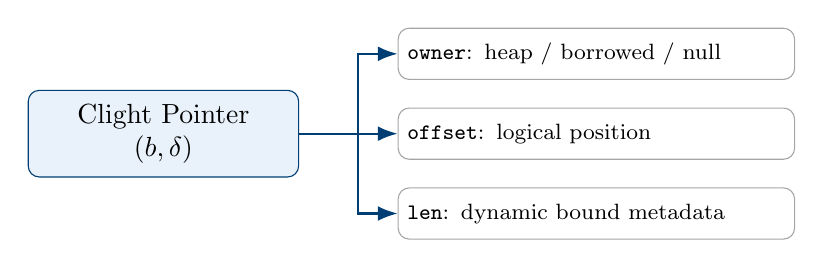
\begin{tikzpicture}[
      node distance=0.35cm and 1.5cm,
      box/.style={rounded corners, draw=SJTUBlue, fill=SoftBlue, minimum height=1.1cm, text width=3.2cm, align=center},
      field/.style={rounded corners, draw=black!35, fill=white, minimum height=0.65cm, text width=4.8cm, align=left, font=\footnotesize},
      arrow/.style={-{Latex[length=2.5mm]}, thick, SJTUBlue}
    ]
      \node[box] (cptr) {Clight Pointer\\$(b,\delta)$};
      \node[field, right=1.25cm of cptr] (offset) {\texttt{offset}: logical position};
      \node[field, above=of offset] (owner) {\texttt{owner}: heap / borrowed / null};
      \node[field, below=of offset] (len) {\texttt{len}: dynamic bound metadata};

      \draw[arrow] (cptr.east) -- ++(0.75,0) |- (owner.west);
      \draw[arrow] (cptr.east) -- (offset.west);
      \draw[arrow] (cptr.east) -- ++(0.75,0) |- (len.west);
    \end{tikzpicture}
  \end{center}

  \vspace{0.2cm}
  \begin{columns}[T]
    \column{0.48\textwidth}
    \begin{block}{Intuition}
      \begin{itemize}
        \item \texttt{owner}: backing storage
        \item \texttt{offset}: current element
        \item \texttt{len}: valid access range
      \end{itemize}
    \end{block}

    \column{0.48\textwidth}
    \begin{exampleblock}{Design payoff}
      \begin{itemize}
        \item movement preserves ownership
        \item aliases share one storage object
        \item access goes through explicit checks
      \end{itemize}
    \end{exampleblock}
  \end{columns}
\end{frame}

\begin{frame}[fragile]{How \ptr{} Is Implemented}
  \small
  \begin{columns}[T]
    \column{0.56\textwidth}
\begin{lstlisting}[language=Rust]
enum Owner<T> {
    Heap(SharedBuffer<T>),
    Borrowed(BaseAddr, Size),
    Null,
}

struct Ptr<T> {
    owner: Owner<T>;
    offset: isize;
    len: usize;
}
\end{lstlisting}

    \column{0.40\textwidth}
    \begin{block}{Three fields}
      \begin{itemize}
        \item \texttt{owner}: who owns the storage
        \item \texttt{offset}: where the pointer is
        \item \texttt{len}: how far access may go
      \end{itemize}
    \end{block}

    \begin{exampleblock}{Core insight}
      \begin{itemize}
        \item aliases share one runtime owner
        \item pointer arithmetic updates only \texttt{offset}
        \item checks are centralized in the runtime
      \end{itemize}
    \end{exampleblock}
  \end{columns}
\end{frame}

\begin{frame}[fragile]{Core Operations of \ptr{}}
  \small
  \begin{columns}[T]
    \column{0.56\textwidth}
\begin{lstlisting}[language=Rust]
alloc(n):
    owner  <- shared(new array[n])
    offset <- 0
    len    <- n

clone(p):
    return Ptr(share(p.owner), p.offset, p.len)

offset(p, k):
    return Ptr(p.owner, p.offset + k, p.len)

load/store(p, i):
    assert p != null
    assert in_bounds(p.offset + i, p.len)
    access p.owner[p.offset + i]
\end{lstlisting}

    \column{0.40\textwidth}
    \begin{alertblock}{Why it works}
      \begin{itemize}
        \item sharing models C-style aliasing
        \item \texttt{offset} models pointer movement
        \item runtime checks replace undefined behavior
      \end{itemize}
    \end{alertblock}

    \begin{block}{Translation reading}
      \begin{itemize}
        \item \texttt{q = p} $\Rightarrow$ \texttt{q = p.clone()}
        \item \texttt{p + i} $\Rightarrow$ \texttt{p.offset(i)}
        \item \texttt{*p} $\Rightarrow$ checked \texttt{load/store}
      \end{itemize}
    \end{block}
  \end{columns}
\end{frame}

\begin{frame}{How C Pointer Operations Become Rust Operations}
  \small
  \begin{tabular}{>{\raggedright\arraybackslash}p{0.24\textwidth} >{\raggedright\arraybackslash}p{0.30\textwidth} >{\raggedright\arraybackslash}p{0.34\textwidth}}
    \toprule
    \textbf{C construct} & \textbf{Meaning in C} & \textbf{Translation idea} \\
    \midrule
    \texttt{p = malloc(n)} & create heap object & \texttt{p = Ptr::alloc(n)} \\
    \texttt{q = p} & create alias & \texttt{q = p.clone()} \\
    \texttt{p + i} & move pointer & \texttt{p.offset(i)} \\
    \texttt{*p} & dereference for read & \texttt{p.load(0)} \\
    \texttt{*p = v} & dereference for write & \texttt{p.store(0, v)} \\
    \texttt{p == NULL} & null test & \texttt{p.is\_null()} \\
    \bottomrule
  \end{tabular}

  \vspace{0.7em}
  \begin{block}{Main message}
    implicit pointer behavior in C is turned into explicit method calls in Rust.
  \end{block}
\end{frame}

\begin{frame}{Why This Abstraction Matters}
  \small
  \begin{columns}[T]
    \column{0.48\textwidth}
    \begin{block}{It preserves three essential C behaviors}
      \begin{itemize}
        \item \textbf{Aliasing}: multiple pointers may observe one mutable object
        \item \textbf{Pointer arithmetic}: movement does not lose the original allocation
        \item \textbf{Lifetime extension}: heap data may outlive inner scopes
      \end{itemize}
    \end{block}
    \column{0.48\textwidth}
    \begin{alertblock}{It also satisfies Rust-side requirements}
      \begin{itemize}
        \item generated logic remains safe Rust
        \item dangerous behavior is isolated in the runtime
        \item invalid access becomes an explicit panic
      \end{itemize}
    \end{alertblock}
  \end{columns}

  \vspace{0.7em}
  \begin{block}{Key Point}
    The real accomplishment of the paper is not the invention of yet another pointer type,
    but the identification of a \good{small, safer, and practical semantic bridge}.
  \end{block}
\end{frame}

\section{Representative Examples}

\begin{frame}[fragile]{Example 1: Mutable Aliasing}
  \begin{columns}[T]
    \column{0.47\textwidth}
    % \textbf{Example from the paper}
\begin{lstlisting}[language=C]
int *p = malloc(2 * sizeof(int));
int *q = p; // q aliases p
q[0] = 1;
return p[0];
\end{lstlisting}
    \column{0.49\textwidth}
    \textbf{Why this is difficult}
    \begin{itemize}
      \item C permits multiple mutable views of the same memory.
      \item Rust's \texttt{\&mut} model does not permit that directly.
      \item A naive use of \texttt{Box} or ordinary cloning destroys the sharing semantics.
    \end{itemize}
  \end{columns}

  \vspace{0.6em}
  \begin{exampleblock}{Translation result}
\begin{lstlisting}[language=Rust]
let mut p: Ptr<i32> = Ptr::alloc(2);
let mut q = p.clone();
q.store(0, 1);
return p.load(0);
\end{lstlisting}
  \end{exampleblock}
\end{frame}

\begin{frame}[fragile]{Example 2: Pointer Arithmetic Must Be Separated from Ownership}
  \begin{columns}[T]
    \column{0.48\textwidth}
\begin{lstlisting}[language=C]
int *p = malloc(2 * sizeof(int));
p = p + 1;
*p = 42;
\end{lstlisting}
    \column{0.48\textwidth}
    \begin{alertblock}{Difficulty}
      \begin{itemize}
        \item In C, the pointer itself may move.
        \item However, the ownership information for the original allocation must not be lost.
        \item A slice- or borrow-based encoding may preserve only the shifted view and lose the original allocation identity.
      \end{itemize}
    \end{alertblock}
  \end{columns}

  \vspace{0.6em}
  \begin{exampleblock}{Translation result}
\begin{lstlisting}[language=Rust]
let mut p: Ptr<i32> = Ptr::alloc(2);
p = p.offset(1);
p.store(0, 42);
\end{lstlisting}
  \end{exampleblock}

  \vspace{0.4em}
  \begin{block}{Takeaway}
    \texttt{offset()} changes only the logical position, not the \texttt{owner}.
    Thus, cursor movement and allocation ownership are explicitly separated.
  \end{block}
\end{frame}


\begin{frame}[fragile]{Why Purely Static Reasoning Fails on Dynamic Offsets}
  
  % 上半部分：左右分栏对比
  \begin{columns}[T, totalwidth=\textwidth]
    \begin{column}{0.48\textwidth}
      {\small\textbf{\color{keywordblue}Original C Code:}}
      \begin{lstlisting}[language=C, basicstyle=\ttfamily\tiny]
void demo(int *arr, int k) {
    int *p1 = arr + 0;
    int *p2 = arr + 5;
    *p1 = 10;
    *p2 = 20;
    int *p3 = p1 + k;
    *p3 = *p1 + *p2;
}
      \end{lstlisting}
    \end{column}
    
    \begin{column}{0.48\textwidth}
      \begin{block}{The Fundamental Difficulty}
        \begin{itemize}\setlength{\itemsep}{1pt}\tiny
          \item \textbf{Static:} \texttt{p1}/\texttt{p2} locations are compile-time known.
          \item \textbf{Dynamic:} \texttt{p3} destination depends on runtime \texttt{k}.
          \item \textbf{Overlap:} Compiler cannot statically check aliasing.
        \end{itemize}
      \end{block}
      
      \begin{alertblock}{Implication}
        \tiny Static splitting alone is insufficient. Runtime safety is necessary.
      \end{alertblock}
    \end{column}
  \end{columns}

  \vspace{0.4em}
  % 使用 Beamer 兼容性最好的画线方式
  \textcolor{lightgray}{\hrulefill}
  \vspace{0.4em}

  % 下半部分：横跨全局的 Rust 翻译结果
  \begin{exampleblock}{Translation Result (Rust)}
    \begin{lstlisting}[language=Rust, basicstyle=\ttfamily\tiny]
let mut p1: Ptr<i32> = arr.clone().offset(0);
let mut p2: Ptr<i32> = arr.clone().offset(5);
p1.store(0, 10);
p2.store(0, 20);
let mut p3: Ptr<i32> = p1.clone().offset(k as isize);
p3.store(0, p1.load(0) + p2.load(0));
    \end{lstlisting}
  \end{exampleblock}

\end{frame}


\section{System Realization}

\begin{frame}{Pipeline Architecture}
  % \centering
  % \begin{tikzpicture}[
  %   node distance=0.95cm and 1.0cm,
  %   box/.style={rounded corners, draw=SJTUBlue, fill=SoftBlue, minimum width=2.0cm, minimum height=0.9cm, align=center},
  %   tool/.style={rounded corners, draw=DeepOrange, fill=SoftOrange, minimum width=2.5cm, minimum height=0.9cm, text width=2.5cm, align=center, font=\scriptsize},
  %   arrow/.style={-{Latex[length=2.4mm]}, thick}
  % ]
  %   \node[box] (csrc) {C Source};
  %   \node[box, right=of csrc] (clight) {Clight IR};
  %   \node[tool, right=of clight] (pass) {\texttt{Clight2Rust}\\\texttt{light.v}};
  %   \node[box, right=of pass] (rustlight) {Rustlight IR};
  %   \node[tool, right=of rustlight] (printer) {\texttt{PrintRust}\\\texttt{light.ml}};
  %   \node[box, right=of printer] (rust) {Rust Source};
  %   \node[tool, below=1.2cm of rust] (runtime) {Runtime Library};
  %   \node[box, right=1.4cm of rust] (exe) {Executable};

  %   \draw[arrow] (csrc) -- node[above] {\scriptsize CompCert} (clight);
  %   \draw[arrow] (clight) -- (pass);
  %   \draw[arrow] (pass) -- (rustlight);
  %   \draw[arrow] (rustlight) -- (printer);
  %   \draw[arrow] (printer) -- (rust);
  %   \draw[arrow] (rust) -- node[above] {\scriptsize \texttt{rustc}} (exe);
  %   \draw[arrow] (runtime) -- (exe);
  % \end{tikzpicture}
  \begin{figure}[htbp]
\vspace{-0.4cm}  
\centering
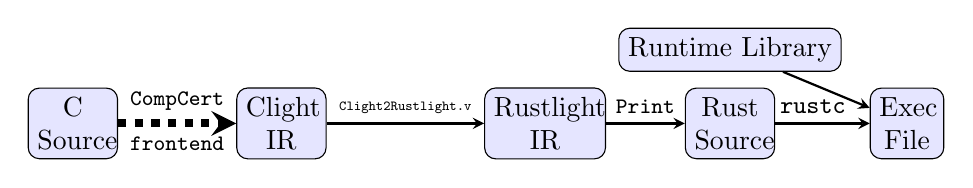
\begin{tikzpicture}[node distance=0.8cm, auto,
    block/.style={rectangle, draw, fill=blue!10, text centered, rounded corners, minimum height=0.5cm},
    arrow/.style={thick,->,>=stealth}]
    
    % --- 主流程节点 ---
    \node [block, text width = 0.9cm] (csrc) {C Source};
    \node [block, text width = 0.9cm, right=1.5 of csrc] (clight) {Clight IR};
    \node [block, text width = 1.3cm, right=2 of clight] (rustlight) {Rustlight IR};
    \node [block, text width = 0.9cm, right=1of rustlight] (rssrc) {Rust Source};
    \node [block, text width = 0.7cm, right=1.2 of rssrc] (binary) {Exec File};
    
    % --- 新增节点：定位在 Rust Source 上方 ---
    % 使用 above=of rssrc 将其放在 Rust Source 正上方
    \node [block, above=of rssrc, above=0.2cm of rssrc] (runtime) {Runtime Library};
    
    % --- 描述文字 ---
    %% \node [text width=2.5cm, align=center, below=0.2cm of clight] {\footnotesize (CompCert Frontend)};
    %% \node [text width=2.5cm, align=center, below=0.4cm of rustlight] {\footnotesize (\textbf{Clight2Rustlight.v})};
    %% \node [text width=2.5cm, align=center, below=0.1cm of rssrc] {\footnotesize (PrintRustlight.ml)};
    
    % --- 箭头连接 ---
    % 1. 主流程
    \draw [arrow, line width = 0.1cm, dashed] (csrc) --
    node[above, font=\footnotesize] {\texttt{CompCert}}
    node[below, font=\footnotesize] {\texttt{frontend}}
    (clight);
    
    \draw [arrow] (clight) --
    node[above, font=\tiny] {\texttt{Clight2Rustlight.v}}
    (rustlight);
    
    \draw [arrow] (rustlight) --
    node[above, font=\footnotesize] {\texttt{Print}}
    (rssrc);
    
    % 2. Rust Source -> Executable (标注 rustc)
    % 为了让标签不重叠，我们可以把标签放在这条线上
    \draw [arrow] (rssrc) -- node[above, pos=0.4, font=\small] {\texttt{rustc}} (binary);
    
    % 3. Runtime Library -> Executable
    % 从上方节点直接指向 binary
    \draw [arrow] (runtime) -- (binary);
    
\end{tikzpicture}

\caption{End-to-end translation pipeline of Clight2Rust}
\label{fig:workflow}
\vspace{-0.7cm}
\end{figure}


  \vspace{0.9em}
  \begin{block}{Two Key Files in the Repository}
    \path{clight2rustlight/Clight2Rustlight.v} defines the translation,
    and \path{rustfrontend/PrintRustlight.ml} prints Rustlight as compilable Rust code.
  \end{block}
\end{frame}

% \begin{frame}{The Meaning of the Translation Rules}
%   \begin{columns}[T]
%     \column{0.53\textwidth}
%     \begin{block}{Representative mappings}
%       \begin{itemize}
%         \item \texttt{Ebinop(Oadd, p, i)} $\Rightarrow$ \texttt{p.offset(i)}
%         \item \texttt{Ederef(p)} $\Rightarrow$ \texttt{p.load(0)}
%         \item \texttt{*p = v} $\Rightarrow$ \texttt{p.store(0, v)}
%         \item \texttt{(*p).f} $\Rightarrow$ load first, then access the field
%       \end{itemize}
%     \end{block}
%     \column{0.43\textwidth}
%     \begin{alertblock}{Why this matters}
%       In C, many memory actions are implicit in syntax.
%       In this framework, they become explicit API calls, so the checking points, trust boundary, and semantic responsibility are all exposed.
%     \end{alertblock}
%   \end{columns}

%   \vspace{0.7em}
%   \begin{exampleblock}{Summary}
%     This is not merely a matter of printing C as Rust syntax.
%     It is a matter of \good{reconstructing implicit C memory actions as explicit, controlled Rust operations}.
%   \end{exampleblock}
% \end{frame}

% \begin{frame}{Why Target Clight?}
%   \begin{itemize}
%     \item Clight is a semantically disciplined subset of C in CompCert, with cleaner structure for expressions, effects, and control flow.
%     \item In Clight, a pointer can naturally be understood as \((b,\delta)\): a block identifier plus an offset. This aligns closely with the design of \ptr{}.
%     \item The goal of the paper is not immediate coverage of all GNU C extensions, but a reliable translation path on a high-assurance subset.
%     \item This also explains the difference from purely engineering-oriented tools: the emphasis is on a \good{credible semantic migration path}, not only on breadth of coverage.
%   \end{itemize}
% \end{frame}

\section{Evaluation and Significance}

\begin{frame}{What Do the Experimental Results Show?}
  \small
  \begin{columns}[T]
    \column{0.48\textwidth}
    \begin{block}{Setup}
      \begin{itemize}
        \item Benchmark suite: CompCert \texttt{test/c}
        \item Reference baseline: C programs compiled by Clang/GCC
        \item The subset of C supports: supports all of the MISRA-C 2004 subset of C
      \end{itemize}
    \end{block}
    \column{0.48\textwidth}
    \begin{exampleblock}{Headline result}
      \begin{itemize}
        \item \good{24/24} benchmarks are translated and executed successfully
        \item Output matches the reference C implementations
        \item Average runtime overhead is approximately \good{1.70x}
      \end{itemize}
    \end{exampleblock}
  \end{columns}

  \vspace{0.7em}
  \begin{tabular}{p{0.26\textwidth}p{0.14\textwidth}p{0.42\textwidth}}
    \toprule
    \textbf{Metric} & \textbf{Value} & \textbf{Interpretation} \\
    \midrule
    Translation success rate & 100\% & all benchmark programs compile and run successfully \\
    Average overhead & 1.70x & memory safety is achieved with a measurable runtime cost \\
    Fastest case & 0.67x & LLVM optimization may outperform the reference C build \\
    Slowest case & 3.36x & dynamic checks become expensive in hot paths \\
    \bottomrule
  \end{tabular}
\end{frame}

\begin{frame}{How Should We Interpret the 1.70x Overhead?}
  \small
  \begin{columns}[T]
    \column{0.48\textwidth}
    \begin{block}{Main sources of overhead}
      \begin{itemize}
        \item the uniform \texttt{load/store} interface
        \item dynamic bounds checking
        \item dynamic borrow tracking in \texttt{Rc<RefCell<...>>}
      \end{itemize}
    \end{block}
    \column{0.48\textwidth}
    \begin{exampleblock}{Why the result still matters}
      \begin{itemize}
        \item It demonstrates that the lightweight runtime-backed route is viable.
        \item The cost is noticeable, but not prohibitive.
        \item More importantly, the work achieves a meaningful balance among safety, automation, and semantic credibility.
      \end{itemize}
    \end{exampleblock}
  \end{columns}
\end{frame}

\section{Limitations and Outlook}

% \begin{frame}{Limitations and the Role of Split Tree}
%   \small
%   \begin{columns}[T]
%     \column{0.48\textwidth}
%     \begin{alertblock}{Current boundary of the work}
%       \begin{itemize}
%         \item The input language is Clight, not arbitrary industrial C.
%         \item Safety depends on a small trusted runtime.
%         \item A full Clight $\rightarrow$ Rustlight semantic preservation proof is not yet complete.
%       \end{itemize}
%     \end{alertblock}
%     \column{0.48\textwidth}
%     \begin{exampleblock}{How to present Split Tree}
%       \begin{itemize}
%         \item as an important static idea in related work
%         \item as a direction for reducing dynamic checking in the future
%         \item as a way to lift part of today's runtime reasoning back into static proof
%       \end{itemize}
%     \end{exampleblock}
%   \end{columns}

%   \vspace{0.7em}
%   \begin{block}{Long-Term Vision}
%     The present \ptr{}-based design answers the question of \good{how to generate safe Rust at all}.
%     The next step is to answer \good{how to recover more static reasoning and reduce runtime overhead and panic points}.
%   \end{block}
% \end{frame}

\begin{frame}{Conclusion}
  \begin{block}{Takeaway}
    The contribution of this paper is not simply the construction of another C-to-Rust translator.
    Its central achievement is to identify and address the most difficult problem:
    \good{how to migrate C pointer semantics into a form that safe Rust can meaningfully represent}.
  \end{block}

  \vspace{0.7em}
  \begin{itemize}
    \item \textbf{Contribution:} it reframes the task as memory-semantic migration.
    \item \textbf{Innovation:} it proposes a practical answer based on \ptr{} and a small trusted runtime.
    \item \textbf{Significance:} it connects verified compiler infrastructure with Rust's safety discipline.
    \item \textbf{Future work:} it opens the way to stronger static reasoning, including Split Tree-style ideas.
  \end{itemize}

  \vspace{0.7em}
  \centering
  \Large Thank you.
\end{frame}

% \appendix

% \begin{frame}[fragile]{Appendix: Rust Code for the Dynamic-Offset Example}
% \begin{lstlisting}[language=Rust]
% fn demonstrate_split_tree(mut arr: Ptr<i32>, mut k: i32) {
%     let mut p1: Ptr<i32> = Ptr::null();
%     let mut p2: Ptr<i32> = Ptr::null();
%     let mut p3: Ptr<i32> = Ptr::null();

%     p1 = arr.clone().offset(0);
%     p2 = arr.clone().offset(5);
%     p1.store(0, 10);
%     p2.store(0, 20);

%     p3 = p1.clone().offset(k as isize);
%     p3.store(0, p1.clone().load(0) + p2.clone().load(0));
% }
% \end{lstlisting}
% \end{frame}

% \begin{frame}{Appendix: Comparison of Three Directions}
%   \scriptsize
%   \begin{tabular}{>{\raggedright\arraybackslash}p{0.22\textwidth} >{\centering\arraybackslash}p{0.14\textwidth} >{\centering\arraybackslash}p{0.22\textwidth} >{\centering\arraybackslash}p{0.15\textwidth} >{\centering\arraybackslash}p{0.17\textwidth}}
%     \toprule
%     \textbf{Direction} & \textbf{Safe Rust} & \textbf{Complex Pointer Coverage} & \textbf{Formal Basis} & \textbf{Cost} \\
%     \midrule
%     Syntactic transpilation & weak & strong & weak & heavy \texttt{unsafe} usage \\
%     Purely static analysis & strong & medium/weak & medium/strong & may reject valid programs \\
%     \papername{} & strong & comparatively strong & strong & runtime overhead \\
%     \bottomrule
%   \end{tabular}
% \end{frame}

\end{document}
